%!TEX root = ../Main.tex


% -----------------------------------------------------------------------------
\section{Implementation}
\label{s:Evaluation}

Stream fusion is ultimately performed for practical reasons. We want the fused result program to run faster than unfused source program.

% -----------------------------------------------------------------------------
\subsection{Finite streams}
\label{s:Finite}

The processes we have seen so far deal with infinite streams, but in practice most streams are finite. Certain combinators such as @fold@ and @append@ only make sense on finite streams, and others like @take@ produce inherently finite output. We have focussed on the infinite stream version as it is simpler to explain and prove, but supporting finite streams does not require substantial conceptual changes.

Unlike infinite streams, pulling from a finite stream can fail, meaning the stream is finished. We therefore modify the @pull@ instruction to have two output labels: one to execute when a value is pulled, and the other to execute when the stream is finished. On the pushing end, we also need some way of finishing streams, so we add a new instruction to close an output stream.

During evaluation we need some way of knowing whether a stream is closed, which can be added as an extra constructor in the \InputState~ type. The same constructor is added to the static input state used by fusion. In this way, for any changes made to evaluation, the analogous static change must be made in the fusion transform.

% For a combinator such as @take@ which only needs a finite prefix of the input stream, it may be useful to add an instruction that allows a pulling process to explicitly disconnect from an input channel. After disconnecting, the process no longer needs to be coordinated with the producer, leaving the producer free to push as often as the other consumers allow. Our implementation supports finite streams, but our mechanized formalization does not cover it.

It is also possible to encode finite streams as infinite streams with an explicit end-of-stream marker (EOF) and case statements. However, this requires the fusion transform to analyse and reason about case statements and their predicates.
% It seems obvious that if two consumers read the same value and check if it is EOF, they will both be the same, but this is undecidable in general.
By making the structure of finite streams explicit and constraining how processes use finite streams, it is not necessary to rely on heuristics for deciding equality of predicates.

% Waffle waffle to get url on its own line
This finite stream extension is described in more detail in the appendix of the extended version of this paper, which is available at \url{http://cse.unsw.edu.au/~amosr/papers/merges.pdf}.

% We now describe the extensions required to support finite streams.
% We add a new @closed@ constructor to the \InputState~ to encode the end of the stream.
% Once an input stream is in the closed state, it can never change to another state: it remains closed thereafter.
% 
% We modify the @pull@ instruction so that it has two output labels (like @case@).
% The first label, the read branch, is executed as before when the pull succeeds and a value is read from the stream.
% The second label, the close branch, is executed when the stream is closed, and no more values will ever be available.
% After a pull takes the close branch, any subsequent pulls from that stream will also take the close branch.
% 
% We add two new instructions for closing output streams and disconnecting from input streams.
% Closing an output stream $(@close@~\Chan~\Next)$ is similar to pushing an end-of-file marker to all readers.
% As with @push@, the evaluation semantics of @close@ can only proceed if all readers are in a position to accept the end-of-file, but instead of setting the new \InputState~ to @pending@ with a value, the \InputState~ is set to @closed@.
% After a stream has been closed, no further values can be pushed.
% 
% Disconnecting from input streams $(@disconnect@~\Chan~\Next)$ signals that a process is no longer interested in the values of a stream.
% This can be used when a process requires the first values of a stream, but does not require the whole stream.
% If a process read the first values of a stream and then stopped pulling, its \InputState~ buffer would fill up and never be cleared, so no other process would be able to continue pulling from that stream.
% Disconnecting the stream allows other processes to use the stream without the disconnected process getting in the way of computation.
% The evaluation semantics for @disconnect@ remove the channel from the inputs of the process.
% After removing the channel from the inputs, when a writing process tries to inject values, this process will just be ignored rather than inserting into the \InputState~ buffer and potentially causing writing to block.
% After a process disconnects from an input channel, it can no longer pull from that channel.
% 
% We also add an instruction for terminating the process (@done@).
% After all input streams have been read to completion or disconnected and output streams closed, the process may execute @done@ to signal that processing is complete.
% 
% The fusion definition must be extended to deal with these new instructions.
% The static input state has a @closed@ constructor added and disconnection is encoded by removal from the input state, and the \ti{tryStep} changes more or less follow the evaluation changes.
% Shared and connected pulls now deal with two more possibilities in the input state: the input may be closed in which case the close branch of the pull is taken; or the other process may have disconnected in which case the pull is executed as in the non-shared non-connected case.
% Connected pushes must also deal with when the other process has disconnected in which case the push is executed as if it were non-connected.
% For @in1@ and @out1@ channels, the new @close@ and @disconnect@ instructions are used as normal with no coordination required.
% For connected @close@, as with @push@, the receiving process must have @none@ and the next step performs the @close@ and sets the input state to @closed@.
% For shared @disconnect@, the @disconnect@ is only performed after both processes have disconnected; otherwise the entry is just removed from the input state.
% For connected @disconnect@, the @disconnect@ is not performed and the entry is removed from the input state.
% 
% Finally, \ti{tryStepPair} is modified so that @done@ is performed when both machines are @done@.
% 
% These modifications allow our system to fuse finite streams as well as infinite.


% -----------------------------------------------------------------------------
\subsection{Benchmarks}
We have implemented this system using Template Haskell in a library called @folderol@\footnote{\url{https://github.com/amosr/folderol}}.
To show practical examples, we use the finite stream extension mentioned in~\S\ref{s:Finite}.
We present three benchmarks: one array algorithm, and two simple file operations.


Quickhull is a divide-and-conquer spatial algorithm to find the smallest convex hull containing all points.
At its core is an operation called `filterMax' which takes a line and an array of points, and finds the farthest point above the line, as well as all points above the line.

We compare against a hand-fused program and a @Data.Vector@ program, which uses shortcut fusion.
The shortcut fusion system cannot fuse both operations into a single loop, and both operations recompute the distances between the line and each point.
% This means a choice must be made: either compute the distances upfront and share them, or recompute the distances in each operation.
% We compared both, and recomputing was significantly faster.
% However, we only benchmarked with two-dimensional points: at higher dimensions, the cost of recomputing distances may outweigh array allocation.

The first group in Figure~\ref{fig:bench:all} shows the runtimes for Quickhull over roughly 80MB of data, or five million points.
The hand-fused version is the fastest, while our version is slower, but still faster than the vector version.
The fact that our version is slower than the hand-fused version is surprising, as the generated GHC core is almost identical: the only difference is an extra continuation bound inside the loop, which acts as a sort of indirect jump in the loop body.
% It is possible that recent work on optimising continuations in GHC~\cite{downen2016sequent} will solve this.

The first file benchmark simply appends two files, while counting the lines.
We compared against three Haskell streaming libraries: Conduit, Pipes, and Streaming.
The second group in Figure~\ref{fig:bench:all} shows the runtimes for appending 2MB of data.
The absolute performance here is poor because all are using line-buffered IO; in practice one would use chunked IO, but the overhead per chunk would remain.

The second file benchmark takes a file and partitions it into two files: one with even-length lines, and one with odd-length lines.
The output lines are also counted.
The three streaming libraries are pull-based, and do not support multiple outputs: the program must be written in a convoluted way or at least partially hand-fused.
Even with hand-fusion, the Pipes and Conduit programs are slower than ours, as well as losing any abstraction benefits from using a streaming library.
The final group in Figure~\ref{fig:bench:all} shows the runtimes for partitioning a 1MB file.



% Fused result programs like the one in Figure \ref{fig:Process:Fused} can be lowered directly to a target language, such as Haskell, C or LLVM abstract assembly. The details of such lowering surely affect the performance of the final program, but as they are largely unrelated to the fusion algorithm itself, we focus on the form of the fused program expressed directly in the process language.


% -----------------------------------------------------------------------------



% -----------------------------------------------------------------------------
%\subsection{Result Size}
%
%As with any fusion system, we must be careful that the size of the result code does not become too large when more and more processes are fused together. The left of Figure~\ref{fig:bench:outputsize} shows the maximum number of output states in the result when a particular number of processes are fused together in a pipelined-manner. To produce this graph we programmatically generated dataflow networks for \emph{all possible} pipelined combinations of the @map@, @filter@, @scan@, @group@ and @merge@ combinators, and tried all possible fusion orders consiting of adjacent pairs of processes. The @merge@ combinator itself has two inputs, so only works at the very start of the pipeline --- we present result for pipelines with and without a @merge@ at the start. The right of Figure~\ref{fig:bench:outputsize} shows the number of states in the result when the various combinations of combinators are fused in parallel, for example, we might have a @map@ and a @filter@ processing the same input stream. In both cases the number of states in the result process grows linearly with the number of processes. In all combinations, with up to 7 processes there are less than 100 states in the result process. 
%%%% AR: Note that the split version also has only one merge?
%
%The size of the result process is roughly what one would get when inlining the definitions of each of the original source processes. This is common with other systems based on inlining and/or template meta-programming, and is not prohibitive.
%
%On the other hand, Figure~\ref{fig:bench:exponential} shows the results for a pathological case where the size of the output program is exponential in the number of input processes. The source dataflow networks consists of N merge processes, N+1 input streams, and a single output stream. The output of each merge process is the input of the next, forming a chain of merges. In source notation the network for N = 3 is @sOut = merge sIn1 (merge sIn2 (merge sIn3 sIn4))@.
%
%When fusing two processes the fusion algorithm essentially compares every state in the first process with every state in the second, computing a cross product. During the fusion transform, as states in the result process are generated they are added to a finite map --- the @instrs@ field of the process definition. The use of the finite map ensures that identical states are always combined, but genuinely different states always make it into the result. 
%
%In the worst case, fusion of two processes produces O($n*m$) different states, where $n$ and $m$ are the number of states in each. If we assume the two processes have about the same number of states then this is O($n^2$). Fusing the next process into this result yields O($n^3$), so overall the worst case number of states in the result will be O($n^k$), where $k$ is the number of processes fused. 
%
%In the particular case of @merge@, the implementation has two occurrences of the @push@ instruction. During fusion, the states for the consuming process are inlined at each occurrence of @push@. These states are legitimately different because at each occurence of @push@ the input channels of the merge process are in different channel states, and these channel states are included in the overall process state.


% -----------------------------------------------------------------------------
\subsection{Optimisation and Drop Instructions}
\label{s:Optimisation}
After we have fused two processes together, it may be possible to simplify the result before fusing in a third. Consider the result of fusing @group@ and @merge@ which we saw back in Figure~\ref{fig:Process:Fused}. At labels @F1@ and @F2@ are two consecutive @jump@ instructions. The update expressions attached to these instructions are also non-interfering, which means we can safely combine these instructions into a single @jump@. In general, we prefer to have @jump@ instructions from separate processes scheduled into consecutive groups, rather than spread out through the result code. The (PreferJump) clauses of Figure~\ref{fig:Fusion:Def:StepPair} implement a heuristic that causes jump instructions to be scheduled before all others, so they tend to end up in these groups.

Other @jump@ instructions like the one at @F5@ have no associated update expressions, and thus can be eliminated completely. Another simple optimization is to perform constant propagation, which in this case would allow us to eliminate the first @case@ instruction. 

Minimising the number of states in an intermediate process has the follow-on effect that the final fused result also has fewer states. Provided we do not change the order of instructions that require synchronization with other processes (@pull@, @push@ or @drop@), the fusibility of the overall process network will not be affected.

% Another optimization is to notice that in some cases, when a heap variable is updated it is always assigned the value of another variable. In Figure~\ref{fig:Process:Fused}, the @v@ and @x1@ variables are only ever assigned the value of @b1@, and @b1@ itself is only ever loaded via a @pull@ instruction. Remember from \S\ref{s:Fusion:FusingPulls} that the variable @b1@ is the stream buffer variable. Values pulled from stream @sIn1@ are first stored in @b1@ before being copied to @v@ and @x1@. When the two processes to be fused share a common input stream, use of stream buffer variable allows one process to continue using the value that was last pulled from the stream, while the other moves onto the next one. 

When the two processes are able to accept the next variable from the stream at the same time, there is no need for the separate stream buffer variable. This is the case in Figure~\ref{fig:Process:Fused}, and we can perform a copy-propagation optimisation, replacing all occurrences of @v@ and @x1@ with the single variable @b1@. To increase the chance that we can perform copy-propagation, we need both processess to want to pull from the same stream at the same time. Moving the @drop@ instruction for a particular stream as late as possible prevents a @pull@ instruction from a second process being scheduled in too early.

% In the result, the interleaved instructions from both source processes then share the same heap variable.  

% In general, the @drop@ for a particlar stream should be placed just before a @pull@ from the same stream. 


\begin{figure}
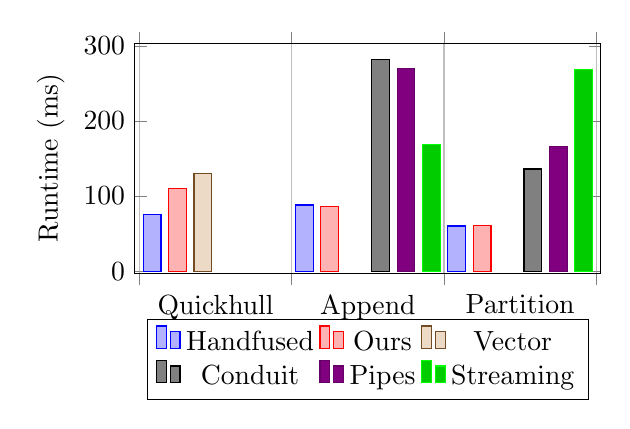
\begin{tikzpicture}
\begin{axis}[
  symbolic x coords={Quickhull, Append, Partition, end},
        ylabel=Runtime (ms),
  ymin=0, ymax=300,
        enlargelimits=0.01,
        ybar interval=0.7,
  width=7.5cm, height=4.5cm,
  legend style={at={(0.5,-0.2)},anchor=north, legend columns=3}
]
\addplot coordinates { (Quickhull, 75) (Append, 88) (Partition, 60) (end, 0) };
\addplot coordinates {(Quickhull, 110) (Append, 86) (Partition, 61) (end,0)};
\addplot coordinates { (Quickhull, 130) (Append, 0)  };
% \addplot coordinates { (Quickhull, 200) (Append, 0) };
\addplot coordinates {  (Append, 282) (Partition, 136) (end,0) };
\addplot coordinates {  (Append, 270) (Partition, 166) (end,0) };
\addplot coordinates {  (Append, 168) (Partition, 268) (end,0) };
\legend{Handfused, Ours, Vector, Conduit, Pipes, Streaming}
\end{axis}
\end{tikzpicture}
\caption{Runtime for benchmarks; lower is faster.}
\label{fig:bench:all}
\end{figure}

% Quickhull
% \addplot coordinates {(200,Store) (130,Recompute) (110,Ours) (75,Hand) (0,end) };
% Append
% \addplot coordinates {(282,Conduit) (270,Pipes) (168,Streaming) (86,Ours) (0,end) };
% Partition
% \addplot coordinates {(1200,Streaming) (764,Pipes) (658,Conduit hand) (288,Ours) (0,end) };

